\section{Theorie}
\label{sec:Theorie}
\subsection{Zielsetzung}
Ziel des Versuches ist es, die Chrarakteristik des \textit{Geiger-Müller-Zählrohrs} zu untersuchen und diese durch seine Funktionsweise zu erklären.

\subsection{Theorie}
\begin{figure}
  \centering
  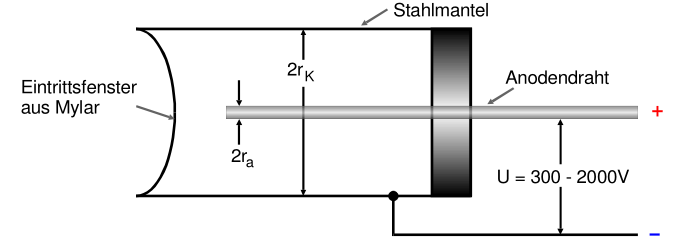
\includegraphics[height=5cm]{./logos/GM.PNG}
  \caption{Schematischer Querschnitt eines Geiger-Müller-Zählrohres \cite{Anleitung}}
  \label{fig:GM}
\end{figure}

Ein Geiger-Müller-Zählrohr besteht im Wesentlichen aus einem metallenen Zylinder mit einem Draht in der Mitte. Zwischen diesen beiden Komponenten wird eine Spannung $U$ angelegt, wobei der Draht aus später beschriebenen Gründen die \textit{Anode} bildet, also positiv geladen wird. Der Hohlraum des Zylinders wird aus mit einem Gasgemisch gefüllt und gasdicht geschlossen, wobei jedoch darauf geachtet wird, dass die Abdeckung auf einer Seite strahlungsdurchlässig ist. Dieser Aufbau ist in \\Abb. \ref{fig:GM} zu sehen. Tritt Strahlung hinreichender Energie in das Zählrohr ein, so kommt es durch Stöße mit dem Füllgas zur Ionisierung. Im anliegenden Feld werden die Elektronen zur Anode beschleunigt, die Ionen zur Kathode (Mantel des Rohres), wobei die Ionen durch die höhere Masse langsamer beschleunigen. Die Elektronen können, wenn sie stark genug beschleunigt werden, weitere Atome ionisieren, wodurch eine \textit{Ladungslawine} entsteht, die das Signal verstärkt. Dies ist der Grund für die Ausrichtung des Feldes. Durch seine Inhomogenität ist das Feld nah am Draht deutlich stärker und auch nah am Draht freigesetzte Elektronen werden noch stark beschleunigt. Durch den Ladungsfluss fließt ein Stromimpuls, der von einem Zählwerk detektiert wird.
Dieser Impuls besitzt allerdings eine gewisse Zeitliche Breite, die \textit{Totzeit} $T$ genannt wird, da während dieser Zeit keine weiteren Impulse detektiert werden können. Da sich durch die Massenträgheit um den Draht positive Ionen stauen, wird das E-Feld teilweise abgeschirmt. \\Dies sorgt dafür, dass die nachfolgenden Impulse geschwächt werden. Nach einer gewissen Zeit (\textit{Erholungszeit} $T_E$) ist dieser Effekt beendet. Der Verlauf der Impulse lässt sich in Abb. \ref{fig:GM-Zeit} betrachten. Die positiven Ionen können durch ihre hohe Masse beim Aufschlag auf den Mantel die Metall-Atome ionisieren und so eine zweite Ladungslawine auslösen, die \textit{Nachentladung} genannt wird. Um  diese Nachentladung zu minimieren wird Alkohol unter das Gas gemischt, der mit seinen langen Molekülketten die Ionen bremst, da die Stöße nun nicht mehr rein elastisch ausgeführt werden, sondern ein Teil der Energie zur Verformung der Kette verwendet wird.

\begin{figure}
  \centering
  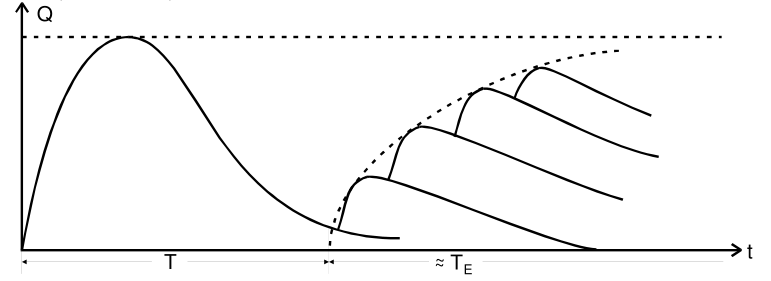
\includegraphics[height=5cm]{./logos/GM-Zeit.PNG}
  \caption{Schematische Darstellung der Ladungsimpulse aufgetragen gegen die Zeit $t$, mit Totzeit und Erholungszeit. \cite{Anleitung}}
  \label{fig:GM-Zeit}
\end{figure}

Da für die Funktion des Geiger-Müller-Zählrohres die Energie der freien Elektronen entscheidend ist, wird im folgenden die Betriebsspannung diskutiert. Zunächst sei hier aus Sicherheitsgründen die \textit{obere Schranke} erwähnt, ab der die anliegende Spannung zur Gasentladung führt und das Zählrohr somit \textit{zerstört}. Sie darf keinesfalls überschritten werden und liegt bei der vorliegenden Apparatur bei über $\SI{700}{\volt}$. Offensichtlich gibt es auch eine untere Schranke, ab der nichts gemessen werden kann, da die Elektronen so wenig beschleunigt werden, dass sie von zentraler liegenden Ionen wieder aufgenommen werden können (\textit{Rekombination}) und so kaum Strom fließt. Ab einem bestimmten Punkt steigt die Anzahl der ionisierten Atome jedoch fast proportional zur anliegenden Spannung, da jedes freie Elektron mit höherer Energie selbst mehr Atome ionisieren kann. Dies ist jedoch nur eine grobe Näherung und geht schließlich in die \textit{Plateau-Phase} über, in der die Zahl der Ionisierungen etwa konstant ist. In diesem Berreich werden üblicherweise die Geiger-Müller-Rohre betrieben. Dieser Verlauf ist in Abb. \ref{fig:GM-Kurve} dargestellt.

\begin{figure}
  \centering
  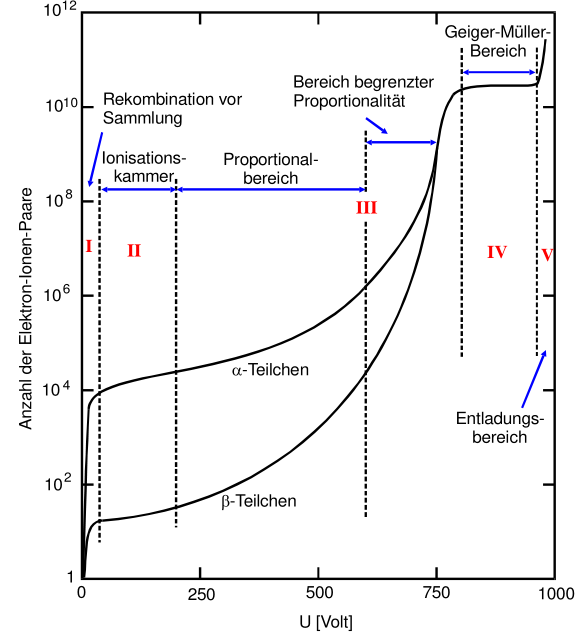
\includegraphics[height = 7cm]{./logos/GM-Kurve.PNG}
  \caption{Anzahl der Elektronen-Ionenpaare aufgetragen gegen die Anliegende Spannung \cite{Anleitung}}
  \label{fig:GM-Kurve}
\end{figure}

Um die Totzeit möglichst exakt zu messen, können zwei Strahlungsquellen (mit Zählraten $N_1$ und $N_2$) überlagert werden ($N_{1+2}$). Ohne Totzeit müsste gelten:
\begin{equation*}
  N_{1+2} = N_1 + N_2.
\end{equation*}
Tatsächlich ergibt sich jedoch
\begin{equation}
  \frac{N_{1+2}}{1- T\cdot N_{1+2}} = \frac{N_1}{1-T\cdot N_1} + \frac{N_2}{1-T\cdot N_2}.
  \label{eqn:2Quellen}
\end{equation}
Gilt $T^2N_i^2<<1$ ,so lässt sich dieser Zusammenhang zu
\begin{equation}
  T \approx \frac{N_1+N_2-N_{1+2}}{2N_1 N_2}
  \label{eqn:easy}
\end{equation}
umformen.
